\documentclass[openright,twoside,10pt]{memoir}
%
% Packages
%
%\usepackage[utf8]{inputenc}
\usepackage[T1]{fontenc}
\usepackage[danish]{babel}
\linespread{1.05}
\usepackage{fontspec}

\setmainfont[Ligatures=TeX]{Garamond}
\setmonofont{Consolas}
% Eksempel
%\newfontfamily{\titlefont}{Antique-Olive Th}

%\newcommand{\heading}[1]{ \vspace{0.5cm} {\titlefont \Large #1}\\ }
%\newcommand{\bilagtitle}[1]{ {\titlefont \LARGE #1}\\ }

%---- 

\usepackage{tocloft}
\usepackage{courier}

\chapterstyle{hangnum}
\raggedbottom
\setlength{\beforechapskip}{0pt}
\setlength{\afterchapskip}{10pt} % vspace under chapters
\setlength{\belowcaptionskip}{-7pt} % vspace mellem caption og tekst
\setsecnumdepth{subsection}

\renewcommand*{\partnamefont}{\normalfont\Huge\bfseries}
\renewcommand*{\partnumfont}{\normalfont\Huge\bfseries}
\renewcommand*{\parttitlefont}{\normalfont\HUGE\bfseries}
\renewcommand*{\chaptitlefont}{\normalfont\HUGE\bfseries}
\setsecheadstyle{\normalfont\huge\bfseries}
\setsubsecheadstyle{\normalfont\Large\bfseries}
\setsubsubsecheadstyle{\normalfont\large\bfseries}

%% Fonts
%\usepackage[sc]{mathpazo}
%\usepackage{courier}
%\usepackage{inconsolata}
%\usepackage[scaled]{uarial}
%\renewcommand*\familydefault{\sfdefault}

% En pil...
\usepackage{textcomp}

\usepackage{multirow}
\usepackage{tabularx}
\usepackage{icomma}
\usepackage{amsmath,amsfonts,amssymb}
\usepackage{mathtools}
\usepackage{graphicx}
\usepackage{gensymb}
\usepackage[usenames,dvipsnames,table]{xcolor} % til farvning af celler i tabel
\usepackage{url}
%\usepackage[bottom]{footmisc} % keep footnotes at bottom UNCOMMENTED
%PGA errors
\usepackage{bbding}
\usepackage{pdfpages}
\usepackage{float} %kan bruge H placement modifier, bedre end "h!"
%\usepackage{wrapfig}
\usepackage{subfig}
%\usepackage{sagetex}
\usepackage[section]{placeins}
\usepackage{xspace}
\usepackage[chapter]{algorithm}
\usepackage{algpseudocode}
\usepackage{algorithmicx}

\parskip=5pt plus 2pt minus 1pt
\parindent=0pt
\frenchspacing % kommeretninger

% Fancy ting med enheder og datatabeller. Læs manualen til pakken
% Manual: http://www.ctan.org/tex-archive/macros/latex/contrib/siunitx/siunitx.pdf
\usepackage{siunitx}

%\usepackage{siunitx}
%\usetikzlibrary{shapes}
\usepackage{enumitem} %stackoverflow.com/questions/3275622/latex-remove-spaces-between-items-in-list
\usepackage{listings}
%\setcounter{secnumdepth}{3}
%\setcounter{tocdepth}{3}

\definecolor{shcomment}{rgb}{0.12, 0.38, 0.18 }
%adjusted, in Eclipse: {0.25, 0.42, 0.30 } = #3F6A4D
\definecolor{shkeyword}{rgb}{0.37, 0.08, 0.25}  % #5F1441
\definecolor{shstring}{rgb}{0.06, 0.10, 0.98} % #101AF9

\setfloatlocations{figure}{htb}

 \lstset{ % http://stackoverflow.com/questions/741985/latex-source-code-listing-like-in-professional-books
%         basicstyle=\footnotesize\ttfamily,% the size of the fonts
                                % that are used for the code
        basicstyle=\footnotesize\ttfamily,% the size of the fonts that are used for the code
         numbers=left,                     % where to put the line-numbers
         numberstyle=\tiny,                % the size of the fonts that are used for the line-numbers
         stepnumber=1,                     % line numbering steps
         numbersep=5pt,                    % how far the line-numbers are from the code
         tabsize=2,                        % sets default tabsize to 2 spaces
         breaklines=true,                  % sets automatic line breaking
         keywordstyle=\color{shkeyword},        % language function text color
    		frame=b,
 %        keywordstyle=[1]\textbf,    % Stil der Keywords
 %        keywordstyle=[2]\textbf,    %
 %        keywordstyle=[3]\textbf,    %
 %        keywordstyle=[4]\textbf,   \sqrt{\sqrt{}} %
         stringstyle=\color{shstring}, % string text color
%         stringstyle=\color{red},
        commentstyle=\color{shcomment},
         showspaces=false,           % show spaces adding particular underscores
         showtabs=false,             % show tabs within strings adding particular underscores   
         showstringspaces=false,     % underline spaces within strings
         xleftmargin=17pt,
         framexleftmargin=17pt,
         framexrightmargin=5pt,
         framexbottommargin=4pt,
         language=Ruby
 }
    %\DeclareCaptionFont{blue}{\color{blue}} 

%\captionsetup[lstlisting]{singlelinecheck=false, labelfont={blue}, textfont={blue}}
\DeclareCaptionFont{white}{\color{white}}
\DeclareCaptionFormat{listing}{\hrule\smallskip\parbox{\textwidth}{\hspace{15pt}#1#2#3}\smallskip\hrule}
\captionsetup[lstlisting]{format=listing,
  singlelinecheck=false, margin=0pt, font={bf,footnotesize}}



\usepackage{memhfixc}
%
% Fra AAU temp
%
\usepackage{calc}
\usepackage{lastpage}

\usepackage{hyperref}
%
% Layout
%
\newenvironment{indledning}{\sffamily}{\vskip 0.75cm}
\newenvironment{tail}{\vskip 0.75cm\itshape}{}
\newcommand{\spc}[1] {#1 \vskip 1cm}
\definecolor{aaublue}{HTML}{0492D2}

\let\oldmarginpar\marginpar
\renewcommand\marginpar[1]{\-\oldmarginpar[\raggedleft\footnotesize #1]%
{\raggedright\footnotesize\color{red} #1}}
% Margins
\setstocksize{11in}{8.5in}
\settrimmedsize{11in}{8.5in}{*}
\settrims{0in}{0in}
\settypeblocksize{9.0in}{6in}{*}
\setlrmargins{1.25in}{*}{*}
\setulmargins{1.0in}{*}{*}
\setheadfoot{14pt}{26pt}
\setheaderspaces{*}{13pt}{*}

% Fra settings.tex
\setlrmarginsandblock{3.5cm}{2.5cm}{*}
\setulmarginsandblock{2.5cm}{3.0cm}{*}

\checkandfixthelayout
%
% Tikz
%
%\tikzstyle{block}=[draw, rectangle, text width=2cm, minimum height=1cm, text badly centered, node distance=\afs]
%\tikzstyle{cloud}=[draw, ellipse, minimum width=2cm, fill=gray!40]
%\tikzstyle{valg} = [draw, diamond, inner sep=1pt, text badly centered, text width=4.5em]
%\tikzstyle{pil} = [draw, -latex]

\setlength{\unitlength}{2em} % for the picture environment

\usepackage[compact]{titlesec}
\titlespacing{\section}{0pt}{*0}{*0}
\titlespacing{\subsection}{0pt}{*0}{*0}
\titlespacing{\subsubsection}{0pt}{*0}{*0}

% Forhindrer horeunger..:

\widowpenalty=300
\clubpenalty=300

\setlength{\parskip}{3ex plus 2ex minus 2ex}

%extra colonner til titelbladet
\usepackage{multicol}

% procenttegn
\let\oldpercent=\%
\renewcommand{\%}{\ifmmode\ \oldpercent\else\oldpercent\fi}

%
% Check-in by Niels on November 07
%
% Alter some LaTeX defaults for better treatment of figures:
    % See p.105 of "TeX Unbound" for suggested values.
    % See pp. 199-200 of Lamport's "LaTeX" book for details.
    %   General parameters, for ALL pages:
    \renewcommand{\topfraction}{0.9}	% max fraction of floats at top
    \renewcommand{\bottomfraction}{0.8}	% max fraction of floats at bottom
    %   Parameters for TEXT pages (not float pages):
    \setcounter{topnumber}{2}
    \setcounter{bottomnumber}{2}
    \setcounter{totalnumber}{4}     % 2 may work better
    \setcounter{dbltopnumber}{2}    % for 2-column pages
    \renewcommand{\dbltopfraction}{0.9}	% fit big float above 2-col. text
    \renewcommand{\textfraction}{0.07}	% allow minimal text w. figs
    %   Parameters for FLOAT pages (not text pages):
    \renewcommand{\floatpagefraction}{0.7}	% require fuller float pages
	% N.B.: floatpagefraction MUST be less than topfraction !!
    \renewcommand{\dblfloatpagefraction}{0.7}	% require fuller float pages



\begin{document}

\setcounter{page}{-100}
\pagenumbering{roman}
\frontmatter
\selectlanguage{danish}
\pagestyle{empty}
\subsection{Forside}
\label{subsec:brug-forside}

Når man taster sig ind på hjemmesiden \url{http://www.foodl.dk}, bliver man mødt af en velkomsthilsen, der meget kort beskriver hjemmesidens formål og brug, som kan ses på \figref{fig:overblik-forside}. Denne hilsen kan brugeren vælge at lukke ned. En cookie bliver gemt i browseren, så velkomsthilsnen ikke bliver vist igen, medmindre browserhistorikken bliver ryddet.

\begin{figure}[H]
	\centering
	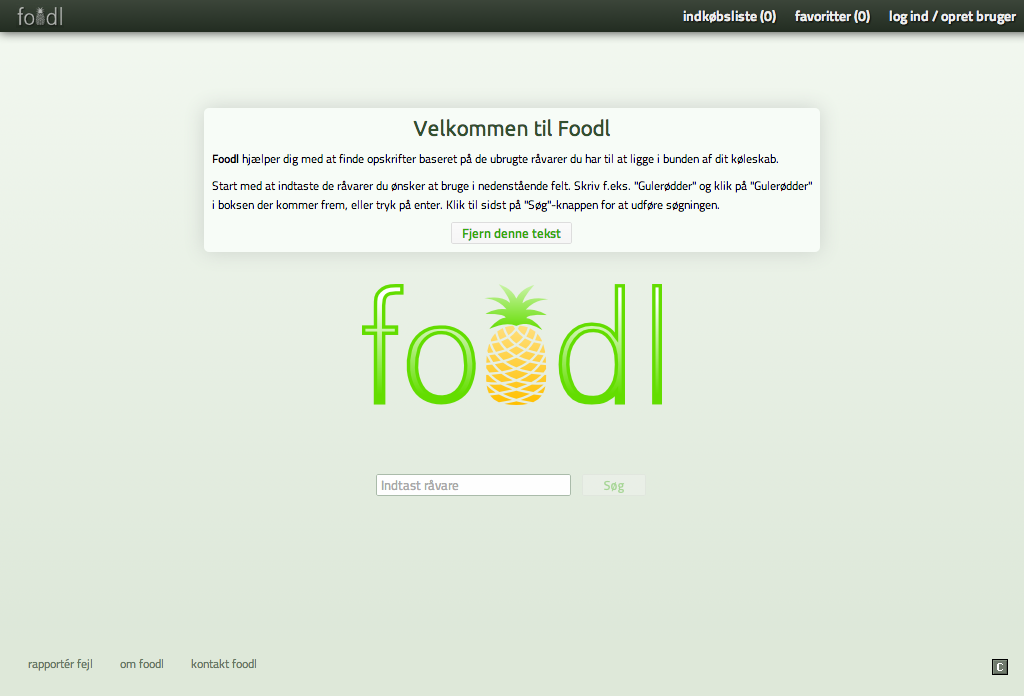
\includegraphics[scale=1]{billeder/foodl/thumbnails/forside.png}
	\capt{Denne figur har til formål at give et overblik over systemets forside.}
	\label{fig:overblik-forside}
\end{figure}

Navnet \Foodl{} er også en del af webapplikationens logo. For at gøre det klarere for en ny bruger, hvad siden handler om, erstattede vi et O i navnet med en stor ananas, fordi det er noget, der kan spises, og sidens formål er at give folk mulighed for at genbruge deres madrester. 

På toppen af alle undersider af \Foodl{} er det muligt at tilgå sidehovedet. Her er der mulighed for at navigere tilbage til forsiden ved at klikke på den mindre version af det store logo. Derudover kan man tilgå både en indkøbsliste, der er nærmere beskrevet i \secref{subsec:brug-indkoebsliste}, og en liste af favorit-opskrifter, som brugeren selv vælger fra hjemmesiden. Favoritlisten bliver beskrevet nærmere i \secref{subsec:brug-favoritliste}. Både indkøbslisten og favoritter har et tal i parentes, der fortæller brugeren, hvor mange varer, der er i den nuværende indkøbsliste, eller hvor mange opskrifter, der er gemt under favoritter. Dette kan ses påtoppen af \figref{fig:overblik-forside}. På sidehovedet kan man også logge ind i systemet eller oprette en bruger, hvilket er forklaret nærmere i \secref{subsec:brug-brugeroprettelse}.

Efter brugeren føler sig tryg ved hjemmesiden og evt. har lukket velkomsthilsnen ned, så er det tid til at indtaste alle de råvarer, der ønskes brugt til madlavningen. Figur \ref{fig:foodl-soegefelt} viser, hvordan en sådan søgning foregår. Der bliver løbende indtastet bogstaver, og systemet undersøger for dele af tekststrenge, der matcher det, som bliver indtastet. Ud fra disse match gives der forslag til hvilke råvarer, man kan vælge. Man kan ikke indtaste, hvad som helst som et søgekriterie i systemet. Der er en lang række råvarer at vælge imellem. Hvis der \fx bliver indtastet kød i søgefeltet, så kommer der en liste af matchende råvarer som forslag, som man kan se på \figref{fig:foodl-soegefelt}. Der er ingen begræsning for, hvor mange råvarer, der kan indtastes som søgekriterier.

\begin{figure}[H]
	\centering
	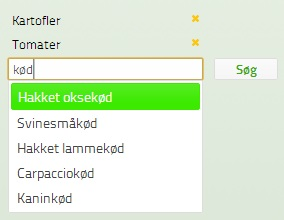
\includegraphics[scale=0.7]{billeder/foodl/soegefelt.jpg}
	\capt{Denne figur viser systemets søgefelt.}
	\label{fig:foodl-soegefelt}
\end{figure}


For at fuldføre en søgning skal man blot trykke på ``Søg'', der er til højre for søgefeltet. Når brugeren trykker ``Søg'', så arbejder systemet på at finde alle de opskrifter, der minimum har én ingrediens, der matcher en af de indtastede råvarer. Det er efter sådan en søgning, at brugeren finder ud af, hvad der er muligt at lave ud fra de råvarer, der er til rådighed (resultatet er afgrænset til den database, man har over opskrifter).
%\clearpage
\begin{nopagebreak}
\LARGE{\textbf{Det Teknisk-Naturvidenskabelige Fakultet}}\vspace{-0.9cm}

\large{\textbf{Datalogi}}
\hspace{10.5cm}
\includegraphics[height=0.75cm]{billeder/aau_logo.pdf}


\hrule

\newcommand{\titleitem}[2]{\textbf{#1:}

\hspace*{0.5cm}
\begin{minipage}{0.9\columnwidth}#2\end{minipage}
\vspace{0.25cm}}
\begin{multicols}{2}

  \titleitem{Titel}{
\includegraphics[width=3.65cm]{billeder/logo.png}\\Anvendelse af Madrester}

\titleitem{Tema}{Udvikling af applikationer – fra brugere til data, algoritmer og test – og tilbage igen}

\titleitem{Projektperiode}{P3, 3. september - 20. december 2012}

\titleitem{Projektgruppe}{d303e12 (\url{d303e12@cs.aau.dk})}

\titleitem{Deltagere}{
    Sebastian Wahl\\
    Simon Buus Jensen\\
    Elias Khazen Obeid\\
    Niels Sonnich Poulsen\\
    Kent Munthe Caspersen\\
    Martin Bjeldbak Madsen
}

\titleitem{Vejleder}{Lise T. Heeager}

% Tilføj senere
% \titleitem{Sidetal}{\pageref{sidsteSideUdenBilag}} 
% \titleitem{Sidetal m/ bilag} {\pgeref{sidsteSideMedBilag}}
\titleitem{Afsluttet}{20. december 2012}

\vfill
\columnbreak

\titleitem{Synopsis}{ Denne rapport gør rede for udviklingsprocessen bag produktionen af systemet \Foodl{}, der er en webapplikation. 
Undersøgelser viser, at personer, der bor i parcelhuse, smider i gennemsnit 42 kg mad ud om året.
\Foodl{} har til formål at gøre det lettere for de madansvarlige i de danske husstande at genbruge madrester fra bl.a. gårsdagens aftensmad for at mindske spildet af mad.

Igennem en iterativ udviklingsmetode har vi analyseret, designet, implementeret og testet systemet.
Vi benyttede en objektorienteret metode, der er blevet præsenteret i bogen Objektorienteret Analyse \& Design \cite{ooad}.
Til udvikling af systemet havde vi et tæt samarbejde med to informanter, der hjalp os med at fortolke og revidere problemstillingen. Informanterne var en stor del af analysen, designet og kvalitetssikringen af systemet.

I konklusionen har vi konkluderet, at \Foodl{} gør det lettere for de madansvarlige at få inspiration til at genbruge madrester.
Vi har, i perspektiveringen, reflekteret over, hvad der kan gøre systemet endnu bedre. }

\end{multicols}
\centering
\textit{Rapportens indhold er frit tilgængeligt, men offentliggørelse (med kildeangivelse) må kun ske efter aftale med
forfatterne.}

\end{nopagebreak}

\cleardoublepage
\pagestyle{ruled}
\section{Forord}

%--Clear page
\newpage
\thispagestyle{empty}
\hspace{1cm}
\newpage
%--

\tableofcontents*
%--Clear page
\newpage
\thispagestyle{empty}
\hspace{1cm}
\newpage
%--

\pagenumbering{arabic}
\mainmatter
\section{Initierende problem}
\label{sec:initierendeproblem}

I Danmark findes der omkring 2,6 millioner husstande \cite{husstande}, der dagligt skal få madlavningen til at gå op i en højere enhed. Der er nemlig mange ting at tage højde for under madlavningen. Der skal tænkes på sundhed for den enkelte, i form af selve kosten, men også sundhed for alle på længere sigt, hvilket opnås ved, at vi i samlet flok skåner miljøet.
En ensformig kost er langt fra lige så sund som en varieret kost. En årsag til ensformighed i madlavningen kan være en travl hverdag, hvor man knytter sig til faste vaner som \fx at lave den samme ret ofte, fordi man synes, den smager rigtig godt og samtidig er lynhurtig at lave. Kosten kan også blive ensformig, fordi man benytter resterne fra madlavningen i nøjagtig samme opskrift dagen efter.
Under madlavningen kan miljøet skånes ved at undgå at smide for meget mad væk. En parcelhusejer smider i gennemsnit 42 kilo spiseligt mad ud om året. \cite{madspildpol} Hvis man ikke vil benytte resterne fra madlavningen i samme opskrift dagen efter, så kan det være svært at finde en ny opskrift at benytte resterne i. I kogebøger bliver det hurtigt uoverskueligt, gang på gang, at blive mødt af opskrifter, der alle kræver en tur i supermarkedet for at få fat på den selleri, man aldrig har. Når man endelig får bevæget sig ned i supermarkedet, så sælges alt i kæmpe portioner. Hakket oksekød findes typisk i pakker med 500 gram som det mindste. Til en enkelt person er dette ofte for meget, og derved risikerer man enten at stå med 100-200 gram hakket oksekød til skraldespanden, eller et problem med hvor dette kød nu skal benyttes. Det er dog muligt at opdele disse store pakker i mindre portioner og fryse dem ned til en anden aften, men tallene for madspild viser, at mange husstande smider meget mad ud, hvilket kan betyde, at de store portioner ikke bliver opdelt i mindre portioner, men blot bliver brugt i madlavningen som de er.

Tal fra Politiken viser, at en parcelhusejer i gennemsnit smider 42 kilo spiseligt mad ud om året. \cite{madspildpol}
Sådanne typer madspild koster desuden danske husholdninger 16 milliarder kroner om året, eller ca. 20 \% af madforbruget af en gennemsnitlig dansk børnefamilie. \cite{madspild16}


% \input{indhold/projektbeskrivelse} \newpage
\chapter{Problemanalyse}
\label{chap:problemanalyse}

\section{Initierende problem}
Mange mennesker vil på et tidspunkt opleve, at deres madlavning begynder at bære præg af ensformighed. Man har et par faste retter, som man er vant til at lave, og i en stresset hverdag er det fristende at holde sig til det, man kender, for at prioritere mere tid til andre ting end madlavning. Vil man dog prøve noget nyt, kan det tage lang tid at bladre en kogebog igennem, før man finder noget, man har lyst til at lave. Ville det ikke være meget lettere med en kogebog, der kun indeholdt de opskrifter, man rent faktisk kunne lave på baggrund af indholdet i ens køleskab. Et stort problem er, at størrelsen på de varer, man køber i supermarkederne, ofte er tilpasset familier på 2-4 personer. Tal fra Politiken og Landbrug \& Fødevarer viser, at en eneboende i gennemsnit smider 98,8 kilo mad ud om året, mens husstande med to personer kun smider 65 kilo ud per person MARTIN KAN IKKE FINDE EN KILDE PÅ DETTE HER EFTER AT LEDE OVERALT (hvor er todo?). Eksempelvis er et halvt kilo oksekød eller en bøtte creme fraiche for meget til én person. Som eneboende står man ofte med et køleskab fyldt med rester, som ikke fik plads i de foregående dages aftensmad. Sådanne typer madspild koster desuden danske husholdninger 16 milliarder kroner om året, eller ca. 20 \% af madforbruget af en gennemsnitlig dansk børnefamilie \cite{madspild16}. 

Kunne man ikke lave en webapplikation, der fungerede som en almindelig kogebog, men som blot viser de opskrifter, man allerede har nogle af ingredienserne til? 

Hvis brugeren har en halv pakke hakket oksekød og en håndfuld tomater, der bliver for gammel i morgen, så ville det være rart at kunne få vist alle de opskrifter, hvor hakket oksekød og tomater indgår. På den måde kunne man undgå madspild og samtidig lave varieret mad på en spændende og kreativ måde.



 \newpage

\section{Problemafgrænsning}
\label{chap:problemafgraensning}

 \newpage
%\input{indhold/problembeskrivelse}

\chapter{Problemløsning}
\label{chap:problemloesning}



\chapter{Konklusion}
\label{chap:konklusion}



 
\section{Perspektivering}
\label{sec:perspektivering}
%problem: madspild - mål:mindske madspild
Formålet med \Foodl{}; at mindske madspild i danske husstande, er ikke et nyt koncept. Vi har undersøgt tre systemer, der bygger på samme idé. Disse har vi forklaret i \secref{sec:eksisterendesystemer}. Systemet er relativt nyt, så der vil højst sandsynligt være mange punkter, hvor der kan ske ændringer, som vil gøre systemet bedre for befolkningen. Her prøver vi at reflektere over, hvordan dette kunne ske.

%flere begrænsningsmuligheder - allergikere
Systemet \Foodl{} implementerer ikke nogle muligheder for \fx allergikere at begrænse søgeresultater til \fx at udelukke opskrifter med nødder eller lignende. Dette kunne være en fornuftig feature at have, hvis man nemt og hurtigt ville have et overblik over de opskrifter, man selv kan have glæde af at lave.

%flere opskrifter
%andre sprog
%involvere flere websider - mindske madspild
Til webapplikationen \Foodl{} har vi kun kontaktet Arla og fået lov til at benytte os af deres, omkring 1000, opskrifter. Ved kun at hente opskrifter fra denne ene side støder vi på nogle ulemper, på grund af de særtræk, der er ved Arlas opskrifter; der er ikke opskrifter nok til at alle råvarer henviser til en opskrift. Enkelte ingredienser er Arlas egne produkter, hvilket giver en anledning til at tro at en lignende ingrediens måske kunne være lige så god eller bedre. Alle opskrifter virker til at være ret krævende med hensyn til antallet af ingredienser der bruges, \fx Arlas opskrift på øllebrød, der udover det basale: øl, brød og sukker, også indeholder kanel, appelsinskal, appelsinsaft og flødeskum. Ved at indhente opskrifter fra flere forskellige opskriftshjemmesider, vil det blive muligt at give brugerne adgang til mange flere opskrifter. Det vil hjælpe på problemet med at ikke alle råvarer er forbundet med en opskrift, og det vil også afhjælpe ulemperne ved de særtræk Arlas opskrifter har. 

Ved kun at benytte Arla som kilde, vil vi få et problem hvis Arlas sider er nede i et par dage. Ved at benytte 100 forskellige kilder, ville vi blot kunne deaktivere søgningen på Arlas opskrifter mens deres side er nede, hvilket ville få minimal betydning blandt 99 andre kilder, sammenlignet med nu, hvor \Foodl{} er afhængig af tilgængeligheden af Arlas hjemmeside.

Madspild forekommer ikke kun i Danmark. Derfor kan man også udvikle systemet til at understøtte andre sprog, og muligvis arbejde sammen med opskriftshjemmesider fra forskellige lande for at kunne levere webapplikationens ydelse til andre lande, der også kunne have gavn af mindre madspild.

%mere intelligent søgningsmetode - flest ud af, hvor mange ingredienser - hvis opskriften har mange ingredienser i forhold til opskrifter med færre ingredienser!
Ser vi på optimering af algoritmer, så skal der være særlig fokus på, hvordan en søgning foretages. På nuværende tidspunkt, så vises søgeresultater, der indeholder ingredienser, der er indtastet af brugeren. Altså den opskrift, der indeholder de fleste matchende ingredienser bliver vist først. Man kunne \fx sortere ud fra hvor stor en procentdel af alle opskriftens ingredienser, der matcher. På denne måde mindsker vi det eventuelle indkøb, der skal til for at lave en opskrift. 

Et eksempel kunne være en søgning på råvarerne kylling og pastinak. Hvis 2 opskrifter fremkommer, den ene med 10 ingredienser og den anden med 25, så vil det, at lave en af opskrifterne, kræve at man skaffer yderligere 8 eller 23 nye råvarer (forudsat man ikke i forvejen har disse). Det ville være smartest at få de opskrifter præsenteret først, der kræver mindst muligt indkøb. Ved at udvikle en mere intelligent søgning, så kan vi også mindske det fremtidige madspild, fordi vi begrænser det eventuelle indkøb af manglende råvarer.

\newpage
	
\bibliographystyle{plain}
\nocite{*} % temp fix for empty 'thebibliography'
\bibliography{kildeliste}


\appendix
%\chapter{Appendiks Eksempel}
\label{ap:eksempel}

\chapter{Fravalgte klasser og hændelser}
\label{ap:fravalgteklasseroghændelser}

Herunder ses de fravalgte klasser, som gruppen ikke finder relevante i forhold til problemområdet. De listes her, da der har været meget diskussion, om hvorvidt klasserne skulle med i systemet eller ej. 

\begin{description}
\item[Person] \hfill \\
Vi vælger at fjerne person-klassen, fordi vi mener, at vores løsning ikke skal være noget socialt media, og derfor mener vi, at det er selve husholdningen, der er fælles om madlavningen selvom det måske blot er en person, der laver mad og står for indkøb og lignende. Brugeren af programmet er ikke en del af problemområdet og skal derfor ikke modelleres som klasse.

\item[Køkken] \hfill \\
Køkken og husholdning dækker over samme del af problemområdet, og vi fjerner derfor køkken og vurderer bagefter om husholdning skal være en klasse.

\item[Husholdning] \hfill \\
En husholdning repræsenterer et hjem, som indeholder én til flere personer. Det er ikke en del af problemområdet at holde styr på eller at kommunikere med andre husstande.

\item[Køleskab/skab/opbevaringsskab] \hfill \\
Om råvarene befinder sig i et køleskab eller i en skuffe er, for os, uinteressant, derfor er vi ikke interesseret i at modellere disse skabe som en klasse.

\item[Køkkenredskab/komfur] \hfill \\
Ligesom ved køleskab/anden opbevaring er vi ikke interesseret i at modellere hvilke redskaber husholdningen har adgang til.

\item[Service] \hfill \\ 
Vi har valgt at fjerne klassen service, fordi denne ikke findes i vores problemområde. Service er noget, der bliver brugt, når man er i færd med at spise det færdige mad, og ikke under selve madlavningen.

\item[Butik] \hfill \\
Vi har valgt at fjerne klassen Butik, da vores system fokuserer på madspild og varieret kost. En modellering af butikker ville være relevant, hvis vores fokus lå på at begrænse udgifter på mad, men da dette imidlertidig ikke er situationen i problemområdet, bliver den udeladt.

\item[Typisk/atypisk ingrediens] \hfill \\
Det er ikke en del af problemområdet at folk ikke er klar over hvilke ingredienser der er normale/unormale at have.

\item[Enhed/Mængde] \hfill \\
Enhed og mængde er ikke klasser, men attributter til en ingrediens.

\item[Madplan] \hfill \\
Informanterne syntes ikke at en madplan var særlig nødvendig. Den indgik i systemdefinition S2, som informanterne fravalgte. Madplanen anses derfor som overflødig, hvorfor denne fjernes som klasse.
\end{description}

\subsection{Fravalgte hændelser}
Fravalgte hændelser ses herunder, da gruppen mener, at det er vigtigt at dokumentere hændelser, der indgik i overvejelser og tidligere klasser. De fravalgte hændelser har en kort forklaring, der beskriver hvorfor en hændelse er blevet fravalgt. Det kan eksempelvis være på grund af, at hændelsen hørte til nogle klasser, som er blevet fravalgt, eller at hændelsen ikke er relevante nok, for de valgte klasser:

\begin{itemize} [noitemsep]
\item Køkkenredskab benyttet (systemet skal ikke holde styr på køkkenredskaber)
\item Råvare benyttet (systemet skal ikke holde styr på mængden af råvarer hos brugeren)
\item Mæthed opnået (fra fravalgte klasser: bruger, person)
\item Madrest opstået (systemet skal ikke behandle råvarer forskelligt om det er rester eller ej)
\item Bord opdækket (fra fravalgt klasse: husholdning)
\item Opvask taget (fra fravalgt klasse: køkken)
\item Service benyttet (fra fravalgt klasse: service)
\item Køleskab åbnet (fra fravalgt klasse: opbevaringsskab)
\item Køleskab lukket (fra fravalgt klasse: opbevaringsskab)
\item Opskrift vurderet (opskrift valgt indebærer, at man har vurderet opskriften)
\item Opskrift anmeldt (ikke en del af problemområdet at anmelde opskrifter)
\item Sult opstået (fra fravalgte klasser: bruger, person)
\item Madlavning afsluttet (fra fravalgte klasser: bruger, person)
\item Madlavning påbegyndt (fra fravalgte klasser: bruger, person)
\item Råvare identificeret (overvåges i form af “råvare købt”-hændelsen med samme resultat)
\item Ingrediens identificeret (indgår i hændelsen opskrift valgt)
\item Madplan lagt (fra fravalgt klasse: Madplan)
\item Madplan startet (fra fravalgt klasse: Madplan)
\item Madplan afsluttet (fra fravalgt klasse: Madplan)
\item Opskrift fravalgt (fra fravalgt klasse: Madplan)
\end{itemize}
\subsection{Fravalgte brugsmønstre}
\label{ap:fravalgtebrugsmoenstre}
\begin{description}
  \item[Skalering] Skalering af ingredienser i opskrifter i forhold til antallet af personer
Fjernet, da skalering indgår i søgningen fordi der er ingen grund til at skalere opskriften i hver visning og kan dermed indgå som en slags “filter” i søgningen.

\item[Råvarehåndtering] Når man gemmer ingredienser i opskrifter... (?)
Fjernet, da råvarehåndtering indgår i søgningen

\item[Overvågning] Hvad skal vi egentligt overvåge?

\item[Begrænsning] \fx ingen kød, glutenfri
Fjernet, da begrænsning indgår i søgningen

\item[Sortering] Sortere opskrifter i forhold til forskellige filtre
Fjernet, da sortering indgår i søgningen

\item[Madplanlægning] Fjernet, da klassen ``madplan'' blev fravalgt i problemområdet

\item[Synkronisering] I stedet for et loginsystem, vil vi benytte cookies og derfor skal synkronisering mellem forskellige enheder håndteres
Vi vælger i stedet et loginsystem, da brugerne er allerede klar over, hvordan sådan et system virker
  
\end{description}
\chapter{Prototyper og møder med informanter}
\label{ap:informant}

\section{Møde 1}

Møde 1 med Merete er blevet optaget\cite{moede1merete}.

\begin{description}
\item[Formål] Igennem et semistruktureret interview med vores to informanter, ønsker vi opnå viden omkring, hvilke problemer informanterne har, i forbindelse med madlavning i det private. På baggrund af denne viden vil vi lave en eller flere systemdefinitioner, som beskriver et eller flere systemer, som vi forventer vil kunne løse disse problemer. 

\item[Spørgmål] Informanterne blev stillet følgende spørgsmål.

\begin{itemize}[noitemsep]
\item Hvad gør du for at undgå madspild?
\item Hvordan planlægger du dine indkøb? Hvordan foregår de?
\item Hvordan finder du ud af, hvad du skal spise til aftensmad?
\item Gør du noget for at spise varieret? (Hvordan/hvorfor ikke?)
\item Beskriv hvordan I i jeres husstand håndterer madlavningen?
\begin{itemize}[noitemsep]
\item Hvem laver mad?
\item Hvem bestemmer hvad I skal have?
\item Hvem køber ind?
\item Hvor tit handler I ind?
\end{itemize}
\item Føler du, at du smider meget mad ud?
\item Laver du en madplan? (hvordan/hvorfor ikke?)
\begin{itemize}[noitemsep]
\item Hvad skal der til for, at du vil anvende en madplan?
\end{itemize}
\end{itemize}

\item[Møde med informant Merete]
Merete bor med sin mand og det er hende, der bestemmer, hvad for noget mad de skal have til aften. Det er altid hende der laver den, men nogle gange kommer manden dog hjem med takeaway.

Merete føler at hun smider meget mad ud. Maden bliver smidt ud når den bliver for gammel, da hun er meget opmærksom på holdbarhedsdatoer. En anden grund til madspild, er at hun før i tiden, har været vant til at lave mad til en hel familie, dengang hendes to sønner og datter boede hjemme, men nu er der kun hende og hendes mand tilbage i husstanden, hvilket har været svært at vænne sig til. Derfor bliver der lavet for store portioner. Hvis mad bliver tilovers, bruges det ofte i en sammenkogt ret næste dag (eksempelvis supper, biksemad osv.).

Merete bruger ikke madplaner af flere grunde. Med en madplan føler de ikke de får særlig meget mad for pengene, da der ikke er nogle madplaner, som tager højde for gode tilbud. Samtidig har Merete og hendes mand et job, som gør at deres planer ofte ændrer sig, og når de er på farten, er det let selv at lave mad, eller at tage højde for en madplan. Hvis Merete skulle bruge en madplan skulle den være baseret på hvad hun har i køleskabet, i en kombination med supermarkedernes gode tilbud. ``Mad leveret til døren''-tilbud fungerer ikke for hende, da hende og manden som før nævnt ofte er på farten, og deres planer ofte ændrer sig impulsivt. Både Merete og hendes mand kan stå for at handle ind. De planlægger sjældent indkøbet, men kan bedre lide at gå på opdagelse efter gode tilbud i forretningen. Merete gør ingenting for at spise varieret, da hun synes det tager for lang tid at tage højde for at få kosten til at blive varieret.

\item[Møde med informant Keld]

Keld bor med sin kone og to døtre ved Østre Anlæg i Aalborg. Han bestemmer, hvad familien skal have at spise hver aften, og han køber ind og laver al maden til familien. Når der bliver lavet mad, så bliver portionen som regel lavet så står, at der er nok til to dage. Familien ønsker nemlig ikke at lave mad hver aften, da der ikke er meget tid i hverdagen. De får oftest spist hele portionen i løbet af to dage, men hvis der bliver noget ekstra tilovers, fryser de den ned, så der bliver smidt så lidt mad ud som muligt. Keld planlægger oftest aftensmad to til tre dage i fremtiden. Når der skal handles ind, så bruges der en indkøbsliste. Dvs., at de har en liste klar, når der skal handles ind. Der kommer oftest også andre sager med i indkøbskurven, fordi de er nemme ofre for impulskøb. Keld handler ca. tre til fire gange om ugen.

Der bliver sjældent spist varieret mad. Det er oftest de samme ``almindelige'' og hurtige danske retter, fordi de har erfaring med disse og de mener, at det er nemt at lave dem. Dvs., at tid er en vigtig faktor, når det kommer til familiens aftensmad. Dog kan det hænde, at der eksperimenteres med nye retter, men dette sker kun i weekenden, når der er lidt ekstra tid.

Madplan er ikke noget, som de bruger, fordi Keld normalvis har en plan i hovedet, som han går efter. Resten af familien har ikke den store indflydelse på madlavningen. Han kommenterer dog, hvis han skulle bruge en madplan, så skulle denne have opskrifter, der ikke tog meget tid, og hvor ingredienserne var håndgribelige. Med dette menes der, at ingredienserne ikke skulle være alt for forskellige, da man pga. af dette ville have sværere ved at mindske sine madrester fra aftensmaden før. Derudover skulle der være nogle billeder til hver opskrift, så man kunne få et hurtigt indblik i hvordan maden skal se ud, og på den måde kan man se, om en opskrift er noget for en. 

\end{description}

\subsection{Sammendrag}
Vi har nu hørt om 2 informanters erfaringer inden for privat madlavning. De 2 informanter har det til fælles, at de begge oplever madspild og ikke benytter en madplan. Netop fordi ingen af informanterne benytter en madplan, kan det være at det blot er en sådan der skal til for at mindske deres madspild. Det kan også være at ingen af dem benytter en madplan fordi de simpelthen ikke kan overtales til dette. For nærmere at undersøge hvordan vi skal løse problemet med madspild, konstruerer vi 2 forskellige systemdefinitioner. Begge systemer forsøger at mindske madspild. Systemdefinition S1 benytter en løsning der ikke involverer en madplan, mens systemdifinition S2 netop benytter en madplan.
\section{Møde 2}

Møde 2 med Merete er blevet optaget \cite{moede2merete}.

Møde 2 med Keld er blevet optaget \cite{moede2keld}.

\cite{moede1merete}.

\begin{description}

\item[Formål]
For at kunne begynde at modellere avendelsesområdet, har vi behov for mere viden om informanternes tanker omkring systemet. En sådan viden vil vi gerne opnå igennem dette møde. Informanterne præsenteres for systemdefinitionerne S1 og S2, hvorefter vi gerne vil høre hvilket system de ønsker at vi skal udvikle. Derefter har vi et par ret lukkede spørgsmål omkring måden de vil bruge systemet på og hvilke funktioner der er nødvendige for at opfylde deres behov.
Mødet med begge informanter er dokumenteret i form af en logbog taget under hvert møde. Derudover kan en optagelse af møderne med Merete\cite{moede2merete} og Keld\cite{moede1keld} findes på de, ved informanternes navne, angivne kilder.

\item[Huskeliste] Listen herunder er en huskeliste for gruppen, når vi skal tale med informanterne.

\begin{itemize}[noitemsep]
\item Præsenter systemdefinition S1 og S2 for informanten
\item Hvor ville du bruge et sådan system? Bærbar, IPhone, Ipad, stationær?
\item Skal programmet kunne huske ingredienser til næste gang, og hvilke ingredienser? Vil du fjerne de ingredienser du bruger under madlavningen?
\item Hvilke opskrifter skal der findes? Forretter, hovedretter, desserter, m.m?
\item Hvordan skal opskrifter sorteres?
\item Retter med eller uden billeder?
\item Andre forslag til programmet?
\end{itemize}

\item[Noter fra møde med Merete]
Merete mener hun helt sikkert ville bruge et program i stil med det nævnt i vores systemdefinition 1. Systemdefinition 2 siger hende ikke rigtig noget. Hun er ret sikker på hun ikke vil bruge en madplan. Hun kan godt lide at have frihed til at lave det hun lige har lyst til. Systemdefinition 1 mener hun vil være nyttigt til at få brugt alle resterne i køleskabet på en smart måde, så de ikke skal smides ud. Hun vil primært bruge programmet på sin bærbar.
Hun ville også bruge programmet selv om hun ingen rester havde, for at få gode idéer til retter hun kan lave.
Køleskabet skal ikke holde styr på ens varelager, hun vil kun bruge programmet inden madlavningen, og ikke efter. Det vil blive for bøvlet hvis man hver gang efter madlavning skal huske at fjerne ingredienser fra programmet. Man har nok at gøre med at rydde op efter maden.
Første gang man bruger programmet skal man kunne indtaste alt hvad man har, også krydderier og mælk. Med en "husk mig" knap, kan man gemme de ingredienser, man ikke vil skrive på hver gang.
Programmet skal kun finde almindelige hverdagsretter, ikke desserter, morgenmad og så videre.
Man skal kunne vælge tilberedningstid. Hvis hun har travlt vil hun ikke have foreslået retter der tager halvanden time at lave. Merete foreslår 3 knapper: 0 - 30 min, 30 - 60 min, > 60 min
En knap at sætte flueben i "Vis mig kun retter uden kød", ville være rar.
Programmet skal sortere opskrifter efter "dem man kan lave", så "dem man mangler 1 ting til", “2 ting til”, osv.
Inden for hver af de netop nævnte lister ville det være rart at kunne sortere efter kalorier, popularitet og tilberedningstid.
Vis kun retter med billeder.

\item[Noter fra møde med Keld]
Jeg forklarede hvordan systemet vil virke efter systemdefinition S1 og S2 og stillede følgende spørgsmål:

\begin{itemize}[noitemsep]
\item Hvad systemdefinition kan du bedst lide? Systemdfinition S1.
\item Hvor ville du bruge sådan et system? Bærbar, mobil, tablet, stationær
\item Skal systemet kunne huske ingredienser til næste gang? Ja
\item Hvilke opskrifter skal der findes? forretter, hovedretter, dessert? Jeg laver normalt ikke forretter og dessert, når vi bare er derhjemme - det er kun, når vi får besøgende
\item Hvordan skal opskrifter sorteres? Årstiden, mængde af passende ingredienser
\item Andre forslag til programmer?
\begin{itemize}[noitemsep]
\item Kommentarer på opskrifter
\item Ingrediensmængdeberegning i forhold til antal personer
\item Printfunktion, så man kan få det på papir
\end{itemize}
\item Retter med eller uden billeder? med billeder!
\end{itemize}

Han lavede tit ensformig mad, når han har tid, kan noget nyt godt laves vha. inspiration fra kogebøger samt internetsider. Info om energi/kulhydrater/vitaminer + mineraler betyder ikke så meget for ham, så længe billedet og opskriften ser lækker og inspirerende ud. Krydderier er ikke vigtige, når man søger på opskrifter.
\end{description}

\subsection{Sammendrag}

\textbf{Enighed blandt begge informanter:}
\begin{itemize}[noitemsep]
\item Systemet bruges på en bærbar
\item Programmet skal fokusere på hovedretter
\item Der skal vises billeder af opskrifterne
\item Opskrifterne skal sorteres efter mængde af passende ingredienser
\item Opskrifter skal kunne skaleres i forhold til personer
\item Systemet skal kunne huske ingredienser til næste søgning
\end{itemize} 

\textbf{Foreslået af enkelt informant:}
\begin{itemize}[noitemsep]
\item Kommentarer på opskrifter
\item Udprinte opskrifter
\item Sorter opskrifter efter årstid, kalorier, tilberedningstid
\item Krydderier er ikke vigtige når man søger på opskrifter
\end{itemize}

\section{Prototype 1}
\label{ap:prototype1}

Afprøvning af Prorotype 1A på Merete er blevet filmet. Klippet kan ses på Youtube: \url{http://youtube.com/watch?v=E-8WA6QrZo4}

Afprøvning af Prorotype 1B på Merete er blevet filmet. Klippet kan ses på Youtube: \url{http://youtube.com/watch?v=rUJexwTpu48}

\begin{description}
\item[Formål] Vores system kan ikke benyttes uden at brugeren indtaster en mængde ingredienser, som de vil udføre en søgning på. For at tilbyde en brugervenlig metode til indtastning af disse ingredienser vil vi gerne teste 2 forskellige metoder på informanterne. Disse 2 metoder testes med hver deres prototype i papirsform, prototype 1A og 1B.
\item[Prototype 1A]

\begin{figure}[H]
\centering
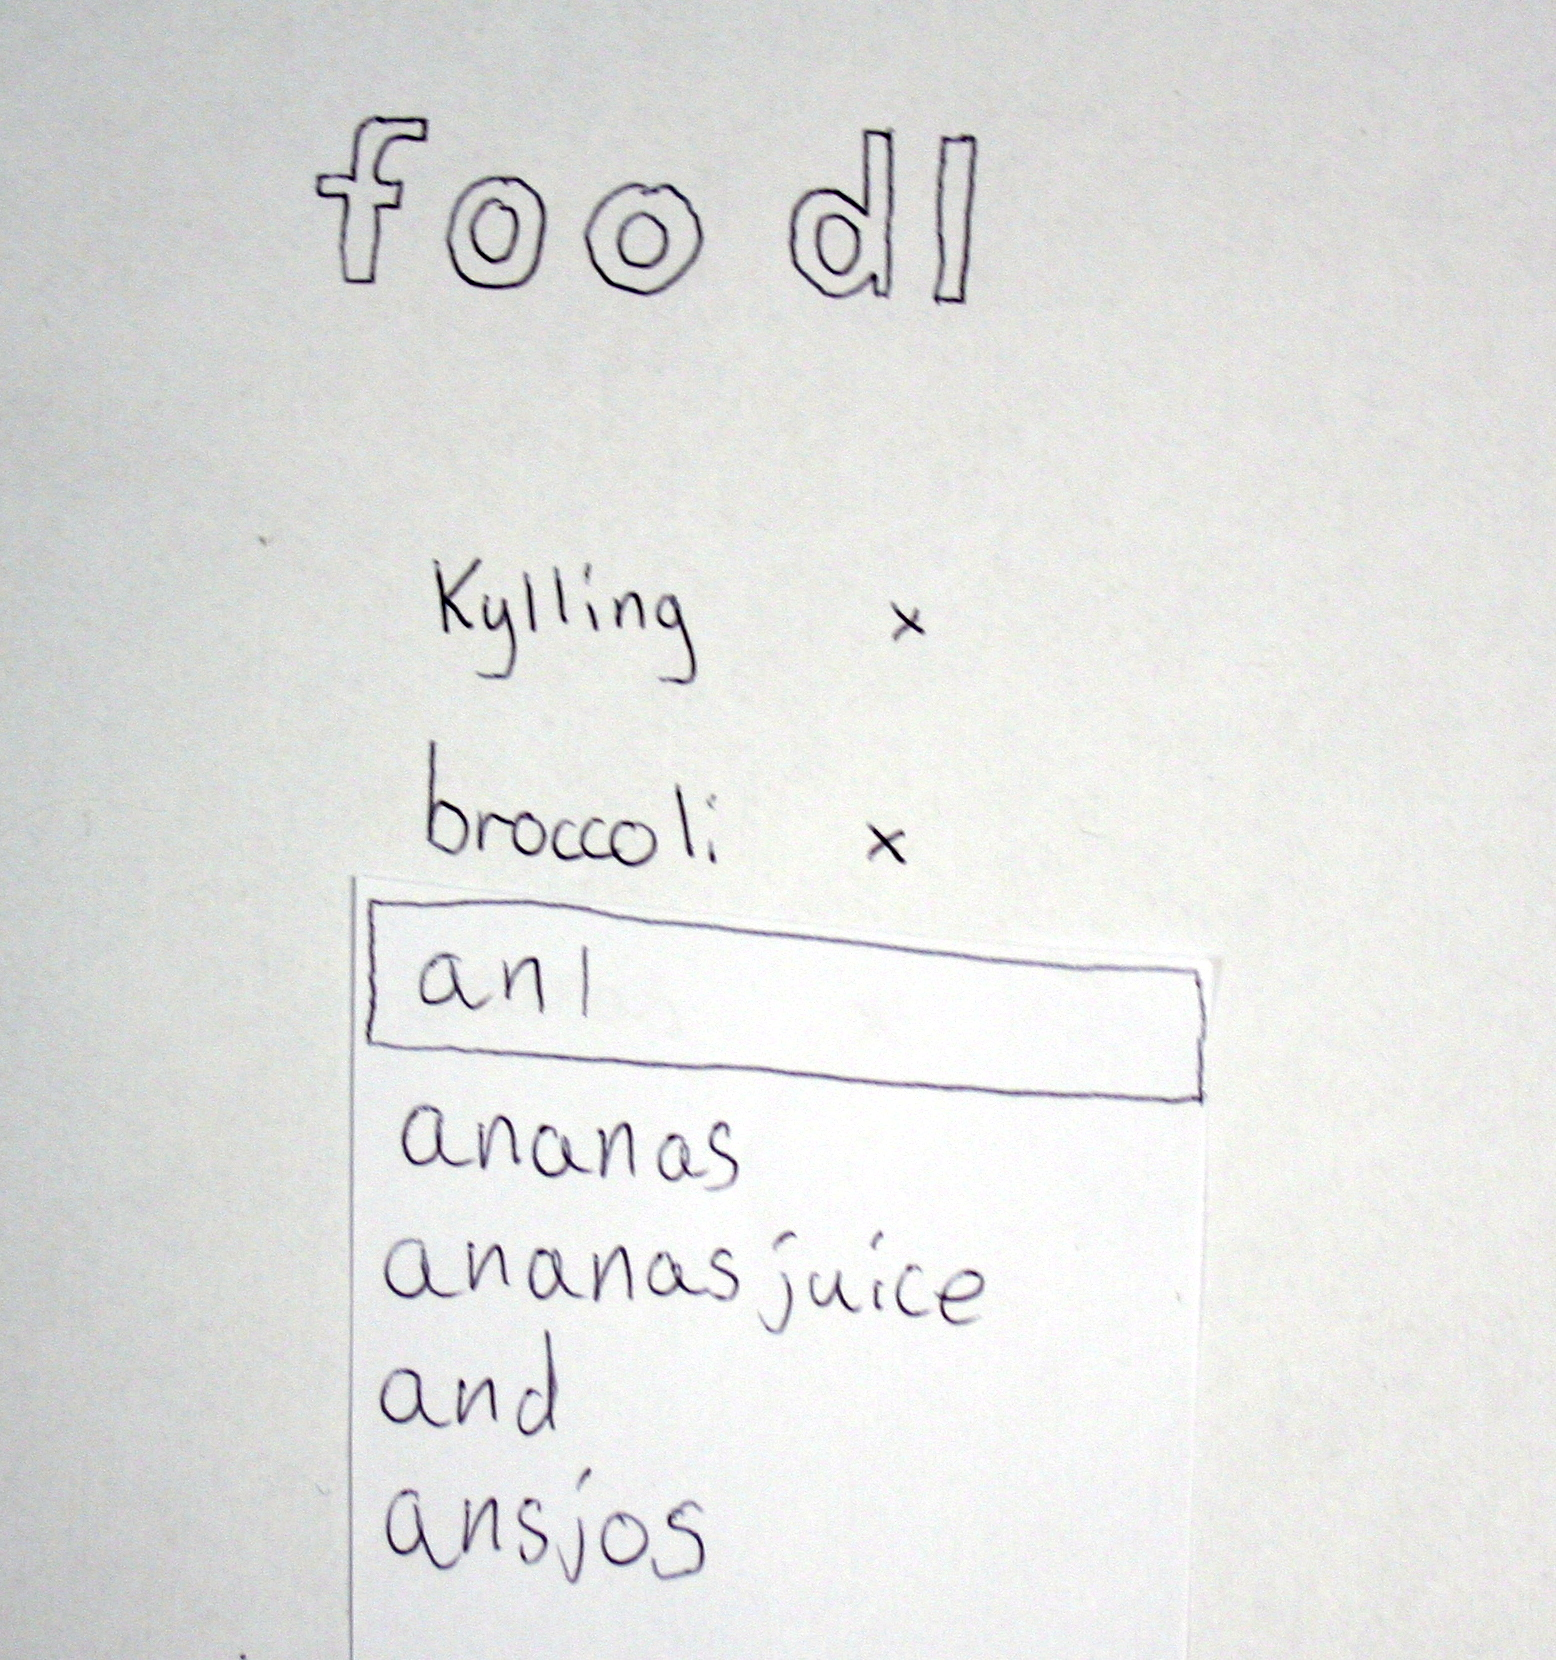
\includegraphics[width=0.5\textwidth]{billeder/prototyper/prototype1a.jpg}
\capt{Visualisering af prototype 1A.}
\label{fig:prototype1a}
\end{figure}

Præsenterer en søgeboks for brugeren, der minder meget om Google’s søgefelt. Når man indtaster et bogstav, fx “k”, kommer der en række forslag frem, såsom kylling og kartoffel, også på samme måde som ved Google, blot med den forskel at der kun foreslås ingredienser. Man kan nu klikke på forslaget eller trykke enter. Man kan også skrive ingrediensens navn færdig manuelt.

Tanken bag denne metode er at man hurtigt kan indtaste en ingrediens hvis man blot ved hvordan de første få bogstaver staves. Brugeren har med stor sandsynlighed kendskab til denne metode, da den bruges af Google, og samtidig har vi også konstrueret logoet og sidens design så det også minder om Google, netop for at gøre det intuitivt for brugeren.

Ulempen er at man har brug for et tastatur og skal tænke over hvordan man staver til ingrediensen. Det er også muligt at overse forslagene og tro man er nødsaget til at stave et meget langt ord, som for eksempel 

\item[Prototype 1B]

\begin{figure}[H]
\centering
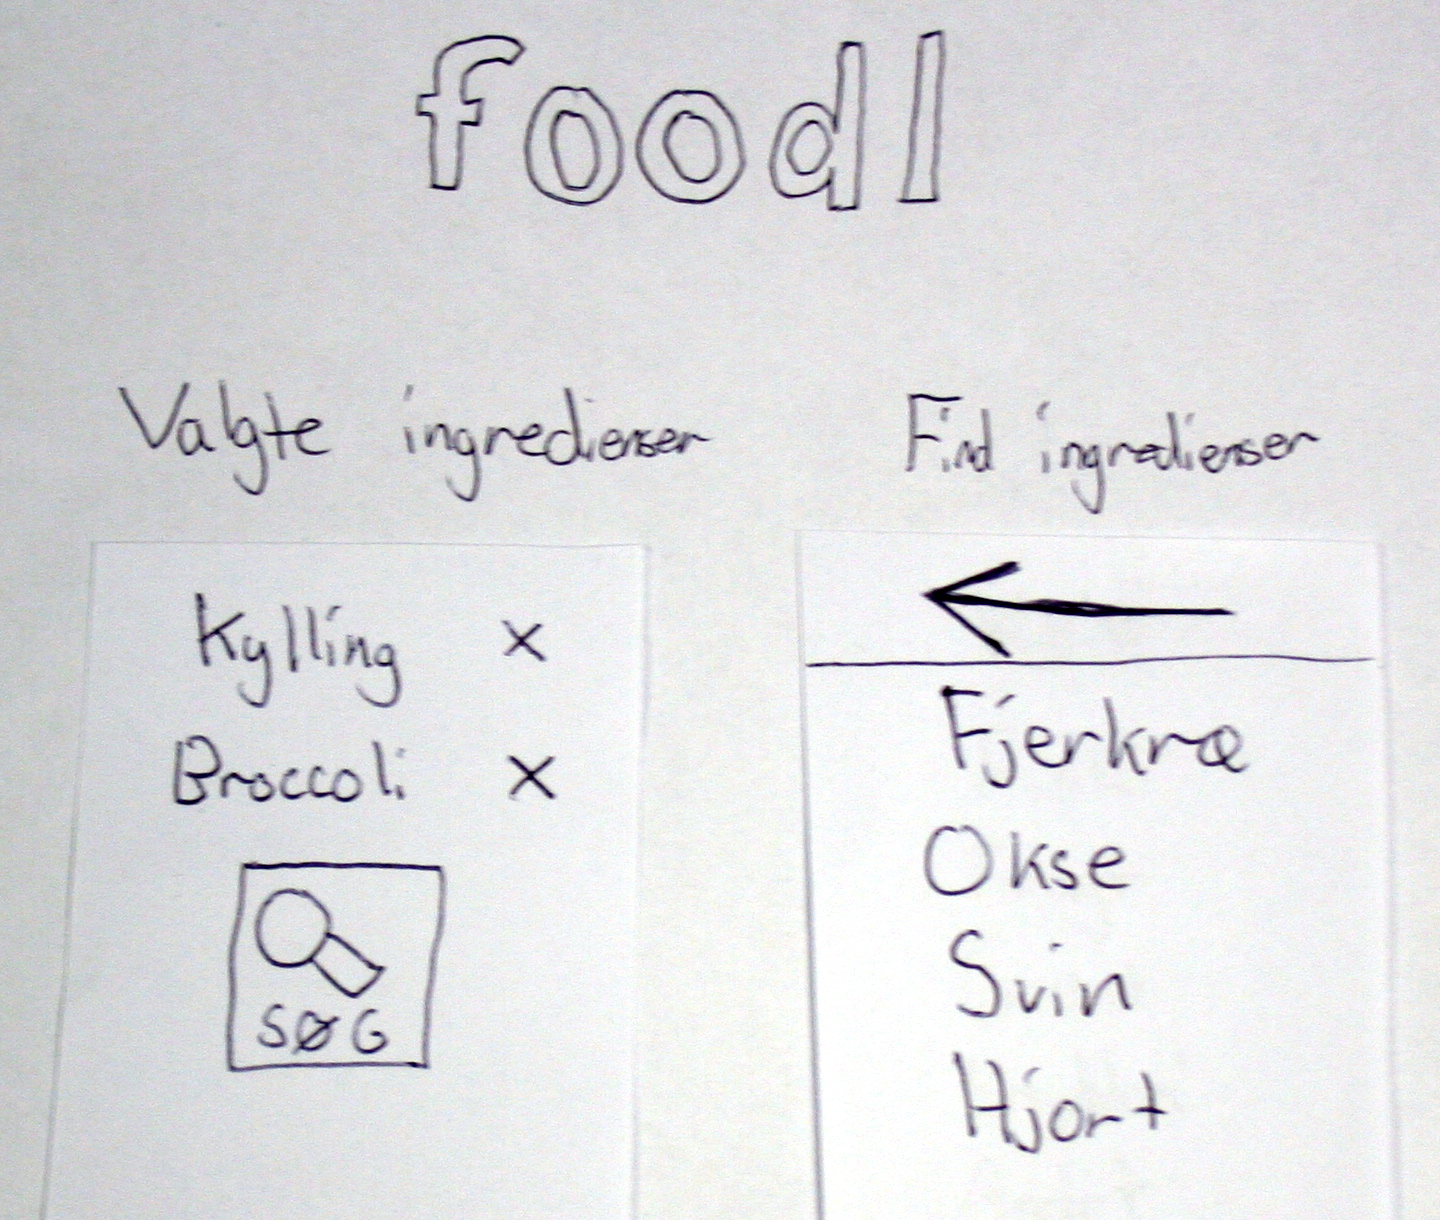
\includegraphics[width=0.5\textwidth]{billeder/prototyper/prototype1b.jpg}
\capt{Visualisering af prototype 1B.}
\label{fig:prototype1b}
\end{figure}

Fokuserer på et valg af ingredienser blandt kategorier. Man vælger først en bred kategori, som for eksempel fjerkræ, kød, brød, frugt og grønt. Dernæst vælger man et antal gange en underkategori, indtil man til sidst kan vælge en ingrediens fra en liste.

Fordelen ved denne metode er at brugeren ikke har behov for et tastatur. Det er også nemt at benytte på tablets og smartphones, da der kan skal klikkes. Ulempen er muligheden for mange kategori og forvirring omkring hvilken kategori en ingrediens findes i. Måske vil den sidste kategori der vælges stadig indeholde rigtig mange ignredienser, sådan at man skal bladre i denne liste for at finde den ønskede ingrediens. 

\item[Sammendrag] Prototype 1A var hurtig, nem og effektiv. Informanten kunne bedst lide denne metode, og hun havde ikke brug for vejledning for at kunne finde de 3 ingredienser kylling, ananas og broccoli.

Prototype 1B var langsommere at bruge og informanten syntes ikke om den. Hun var i tvivl om hvilken kategori hun skulle vælge kylling under. Kategorierne kan laves på mange forskellige måder, og uanset hvordan de vælges, vil der med garanti være nogle brugere der er i tvivl om hvor de skal lede efter en bestemt ingrediens. Et eksempel kan være kartoffelstivelse. Nogle vil lede efter kartoffelstivelse i kategorien grøntsager (fordi kartofler findes der), mens andre måske vil lede efter en kategori med navnet brød og gryn.

På baggrund af informantens valg, vælger vi at benytte metoden fra prototype 1A til at vælge ingredienser.
\end{description}

\section{Prototype 2}

Afprøvning af prototype 2 m/ fokus på systemets funktioner

\begin{description}
\item[Formål] På baggrund af møde 2, hvor informanterne kom med krav til systemets funktioner, har vi nu lavet en diasshow-prototype på gomockingbird.com, hvor systemets funktion er vist. Når informanterne præsenteres for funktionerne i noget der, med lidt god vilje, ligner et rigtigt program, så kan det være at informanten bliver klar over at en funktion enten mangler, eller at en tidligere foreslået funktion er overflødig. Formålet med mødet er derfor primært at ud af, om der er de funktioner, som informanten har brug for. Derudover vil vi også gerne finde ud af om brugeren kan finde de nødvendige funktioner, altså om programmet og dets funktioner som helhed er intuitive at bruge for informanterne.

\begin{figure}[H]
\centering
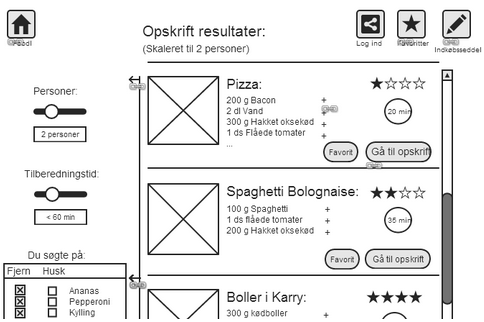
\includegraphics[scale=0.7]{billeder/prototyper/prototype2.png}
\capt{Visualisering af prototype 2.}
\label{fig:prototype2}
\end{figure}

Først udføres en case for at få ledt brugeren rundt blandt alle funktionerne.

\item[Case] Følgende case blev udført af informanterne.

\begin{enumerate}[noitemsep]
\item Udfør en søgning på ingredienserne (pepperoni, ananas og kylling). Ingredienser tilføjes ved at klikke i søgefeltet
\item Skjul alle opskrifter med nødder
\item Gå til den første opskrift, der fremkommer
\item Gå tilbage og tilføj 200 g Bacon (fra pizzaens ingredienser) til din indkøbsliste
\item Print indkøbslisten ud
\item Gør klar til en helt ny søgning
\item Foretag en søgning på pepperoni
\item Du fandt ingen opskrifter, så du vil gerne tilføj ananas, inden du søger igen (du søger altså på pepperoni og ananas)
\item Føj den første opskrift, du finder, til dine favoritter
\end{enumerate}

Efter casen tages en snak om hver af disse funktioner og muligheder med systemet.

Informanten bliver præsenteret for mange funktioner, hvor vi her beskriver hvad deres mening var omkring disse funktioner efter at have udført casen.

\begin{itemize}[noitemsep]
\item Begrænse søgeresultat efter tilberedningstid
\begin{itemize}[noitemsep]
\item Merete synes idéen er god, men foreslår nu kun 2 valgmuligheder ``kort'' eller ``lang'' tilberedningstid
\item Keld synes også dette er en god ide. En opdeling på en 30 min. burde være fint, måske 15 min. Hvis det er tilberedningstid på over en time, må skalaen godt springe mere end 15-30 min.
\end{itemize}
\item Sidebar
\begin{itemize}[noitemsep]
\item Merete opdagede ikke at denne sidebar kunne trækkes ud
\item Den ligger ikke logisk for en. Selvom den er stor. Den bliver skjult i designet
\item Keld synes ikke det ser for rodet ud, selvom sidebaren er ude hele tiden
\end{itemize}
\item Skalere en opskrift til x personer
\begin{itemize}[noitemsep]
\item Merete ser det som en nyttig funktion, hun vil skalere til mellem 2-4 personer
\item Det er en god funktion, som Keld er sikker på mange vil få brug for. Opskalering til 5 burde være nok. Måske 1-20, så er gæstebehov også dækket ind. Men det er trods alt til rester, så til 5 personer burde være nok.
\end{itemize}
\item Fjerne ingredienser inden en søgning udføres (på forsiden)
\begin{itemize}[noitemsep]
\item Merete synes det er meget brugbart
\item Keld synes det er fint at det er på forsiden
\end{itemize}
\item Fjerne ingredienser efter en søgning er udført (på søgeresultatsiden)
\begin{itemize}[noitemsep]
\item Merete synes idéen med at kunne fjerne ingredienser mens der vises søgeresultater er god
\item Keld synes det er fint, at det også er muligt i sidebaren
\end{itemize}
\item Huske ingredienser til næste søgning
\begin{itemize}[noitemsep]
\item Merete synes måden det fungerer på i prototypen er god. Hun vil ikke have at de huskede ingredienser vises på forsiden
\item Keld synes det er rart at det er muligt at huske nogle ingredienser. Det ville måske også være rart, hvis det også var muligt at gøre fra forsiden. Keld er dog i tvivl om, hvor på forsiden det skulle være. Det er måske alligevel bedst hvis forsiden er simpel. Han synes funktionen er brugbar
\end{itemize}
\item Skjule opskrifter indeholdende bestemte ting
\begin{itemize}[noitemsep]
\item Merete synes det virker godt
\item Keld synes det er en god ide. Han fik hurtigt fundet funktionen, så snart toolboxen blev åbnet
\end{itemize}
\item Browsers tilbageknap går til forsiden (beholder ingredienser)
\begin{itemize}[noitemsep]
\item Merete opdagede ikke denne funktion
\item Keld opdagede funktionen, og anvendte den også. Måske ville en tilbage- og fremknap på selve siden være brugbar, foreslår Keld
\end{itemize}
\item Home knap går tilbage (fjerne ingredienser)
\begin{itemize}[noitemsep]
\item Merete synes det virkede naturligt
\item Keld synes det er godt at have en kanp som går helt tilbage. Men han foreslår endnu engang at have en frem- og tilbageknap som supplerer home-knappen
\end{itemize}
\item Visning af opskrifter (ekspander ved mouse over)
\begin{itemize}[noitemsep]
\item Merete synes opskrifterne blev vist fint. Hun kunne godt lide idéen med at ekspandere opskriften ved mouseover
\item Keld synes bare man skal have vist de væsentligste ingredienser. Han synes det ville være smart, hvis det var muligt at se hele ingredienslisten ved hjælp af et mouse-over
\end{itemize}
\item Gå til opskrifter (evt link ved klik på navn)
\begin{itemize}[noitemsep]
\item Merete synes ikke knappen “Gå til opskrift”, er overflødig. Hun ville blive forvirret hvis den ikke var der, og man bare skulle trykke et sted på opskriften (navnet, eller baggrunden, hvor baggrundsfarve ændrer sig eller lignende)
\item Keld synes det er godt med en “Gå til opskrift”-knap. Det er brugervenligt
\end{itemize}
\item Tilføj opskrift til favoritter
\begin{itemize}[noitemsep]
\item Merete synes ikke man skal gå fra et søgeresultat og over til favoritsiden hver gang man tilføjer en opskrift til favoritter. Opskriften skal blot tilføjes. Måske den skal sige en lyd og fjerne knappen man trykkede på. Favoritter-ikonet kunne lyse op
\item Skal lave en “Fjern fra favorit-knap”, så man hurtigt kan ombestemme sig
\item Keld synes det er smart nok at man sendes ind på favoritlisten, så man er sikker på at opskriften er kommet derind. Havde man samtidig en frem- og tilbageknap ville det være endnu bedre
\end{itemize}
\item Favoritter (knappen, der viser ens favoritter)
\begin{itemize}[noitemsep]
\item Merete var lidt forvirret med hensyn til om den tilføjede en opskrift til favoritter, eller hvad den gjorde
\item Keld synes at det skal være muligt at skalere opskrifterne på favoritsiden og at det er muligt nemt at fjerne opskrift fra favoritsiden igen
\end{itemize}
\item Visning af favoritter (layout)
\begin{itemize}[noitemsep]
\item Merete syntes layoutet var godt, og kunne godt lide at det mindede om layoutet ved visning af søgeresultat
\item Keld synes godt om layoutet
\end{itemize}
\item Visning af indkøbsliste
\begin{itemize}[noitemsep]
\item Merete synes det er en god idé at man kan tilføje tekst
\item Keld foreslår at man har ingredienslisten fra den opskrift man har været inde på, ved siden af indkøbslisten, så det er muligt hurtigt at tilføje flere ingredienser derfra
\item Keld synes indkøbslisten er meget brugbar. Det er for ofte man glemmer nogle ting, uden indkøbslisten
\end{itemize}
\item Tilføje opskrifts ingredienser til indkøbsliste
\begin{itemize}[noitemsep]
\item Merete vidste ikke hvordan man gjorde. Hun troede ikke man kunne trykke på +’et
\item Keld kunne godt tilføje en ingrediens til indkøbslisten
\end{itemize}
\item Home-knappen sender en til en helt tom forside
\begin{itemize}[noitemsep]
\item Merete kunne godt lide dette. Det virkede helt naturligt for hende
\item Keld synes det giver mening
\end{itemize}
\item Logge ind (få afklaret med brugeren, hvordan det skal foregå)
\begin{itemize}[noitemsep]
\item Log ind mest forståeligt
\item Kender meget til login, intet til synkronisering
\item Log ind er klart mest forståeligt for Keld. Keld har ikke lyst til at indtaste mere end mail-adresse, navn eller brugernavn og adgangskode. Helst ikke mere end det. Det er fint at der kommer en bekræftelsesmail til ens indbakke, men helst ikke aktiveringsmail
\item Sikkerheden har ikke høj-prioritet for Keld, da der alligevel ikke er nogle følsomme informationer på siden
\end{itemize}
\item Informants forslag til flere funktion
\begin{itemize}[noitemsep]
\item Merete havde ingen forslag, udover at der skal være billede af opskrifterne, hvilket ikke var vist i prototypen
\item Keld foreslår at sidebaren også er på favoritsiden
\item Keld foreslår en frem- og tilbageknap
\item Filtrering af forskellige landes køkkener, så det eksempelvis var muligt at se italienske retter, kinesiske retter osv. (kun de mest kendte køkkener: nordiskekøkken, kinesiske, italienske, græske \fx)
\end{itemize}
\end{itemize}
\end{description}

\subsection{Sammendrag}

I forhold til funktionalitet i prototypen, er der nogle få ting, der skal tilføjes, fjernes eller ændres

\begin{enumerate}[noitemsep]
\item Når man på søgesiden tilføjer en opskrift til favoritter, skal man forblive på søgesiden. Knappen man trykkede på skal erstattes med en ``Fjern fra favoritter''-knap
\item Sidebaren på søgeresultatssiden skal være nemmere at få øje på. En løsning er at gøre den synlig fra starten og give brugeren muligheden for at skjule den
\item Knappen i toppen, der viser de favoritter man har gemt, skal være mere sigende. ``Vis favoritter'' kunne der stå under den
\item På søgeresultatsiden, hvor en opskrifts vises, skal +’et ud for ingredienserne, der tilføjer en ingrediensen til indkøbslisten, være mere intuitiv
\item Brugeren skal muligvis have at vide, at man kan benytte browserens tilbageknap for at gå tilbage til forsiden, uden at ingredienser fjernes. Det kan være at informanten overså denne funktion fordi prototypen blev vist i form af et diasshow på en hjemmeside, og informanten derfor var bange for at gå væk fra hele diasshowets side
\item Skalering og andre funktioner til visning af favoritter
\item Frem og tilbage knap, der giver brugeren tryghed når han navigerer rundt, så man ikke skal være bange for at browseren forsvinder fra siden
\end{enumerate}

%\section{Supplerende spørgsmål}

Her findes spørgsmål, der løbende er blevet stillet informanterne, ved tvivlstilfælde udenfor planlagte møder.

Formål: At afklare om klassen indkøbsliste i problemområdet skal aggregere en råvaretype-, en ingrediensklasse eller begge dele.
Os: ``Lad os sige, at du har fundet en opskrift du gerne vil købe ind til. Du beslutter dig for at lave en indkøbsliste, så du kan huske hvad du skal købe for at lave opskriften. Vil du skrive på indkøbslisten, hvor meget du skal købe af de forskellige ingredienser?''
Merete: ``Ja, det vil jeg helt klart, ellers ville jeg være bange for at glemme hvor meget jeg har brug for.''


\chapter{Manuel mapping}
\label{ap:manuel-mapping}

\begin{figure}
\centering
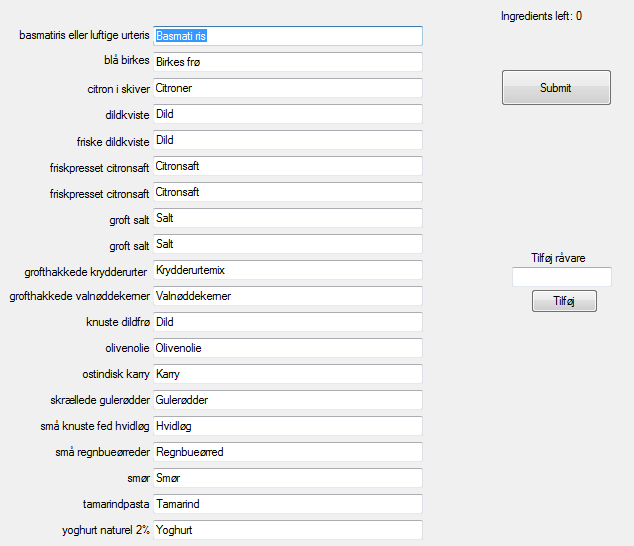
\includegraphics[scale=0.6]{billeder/manuel-mapping.png}
\capt{Program skrevet i C\# til kontrol og remapping af ingredienser}
\end{figure}


\chapter{Valg af mapping metode}
\label{ap:valgafmappingmetode}

\begin{figure}
\centering
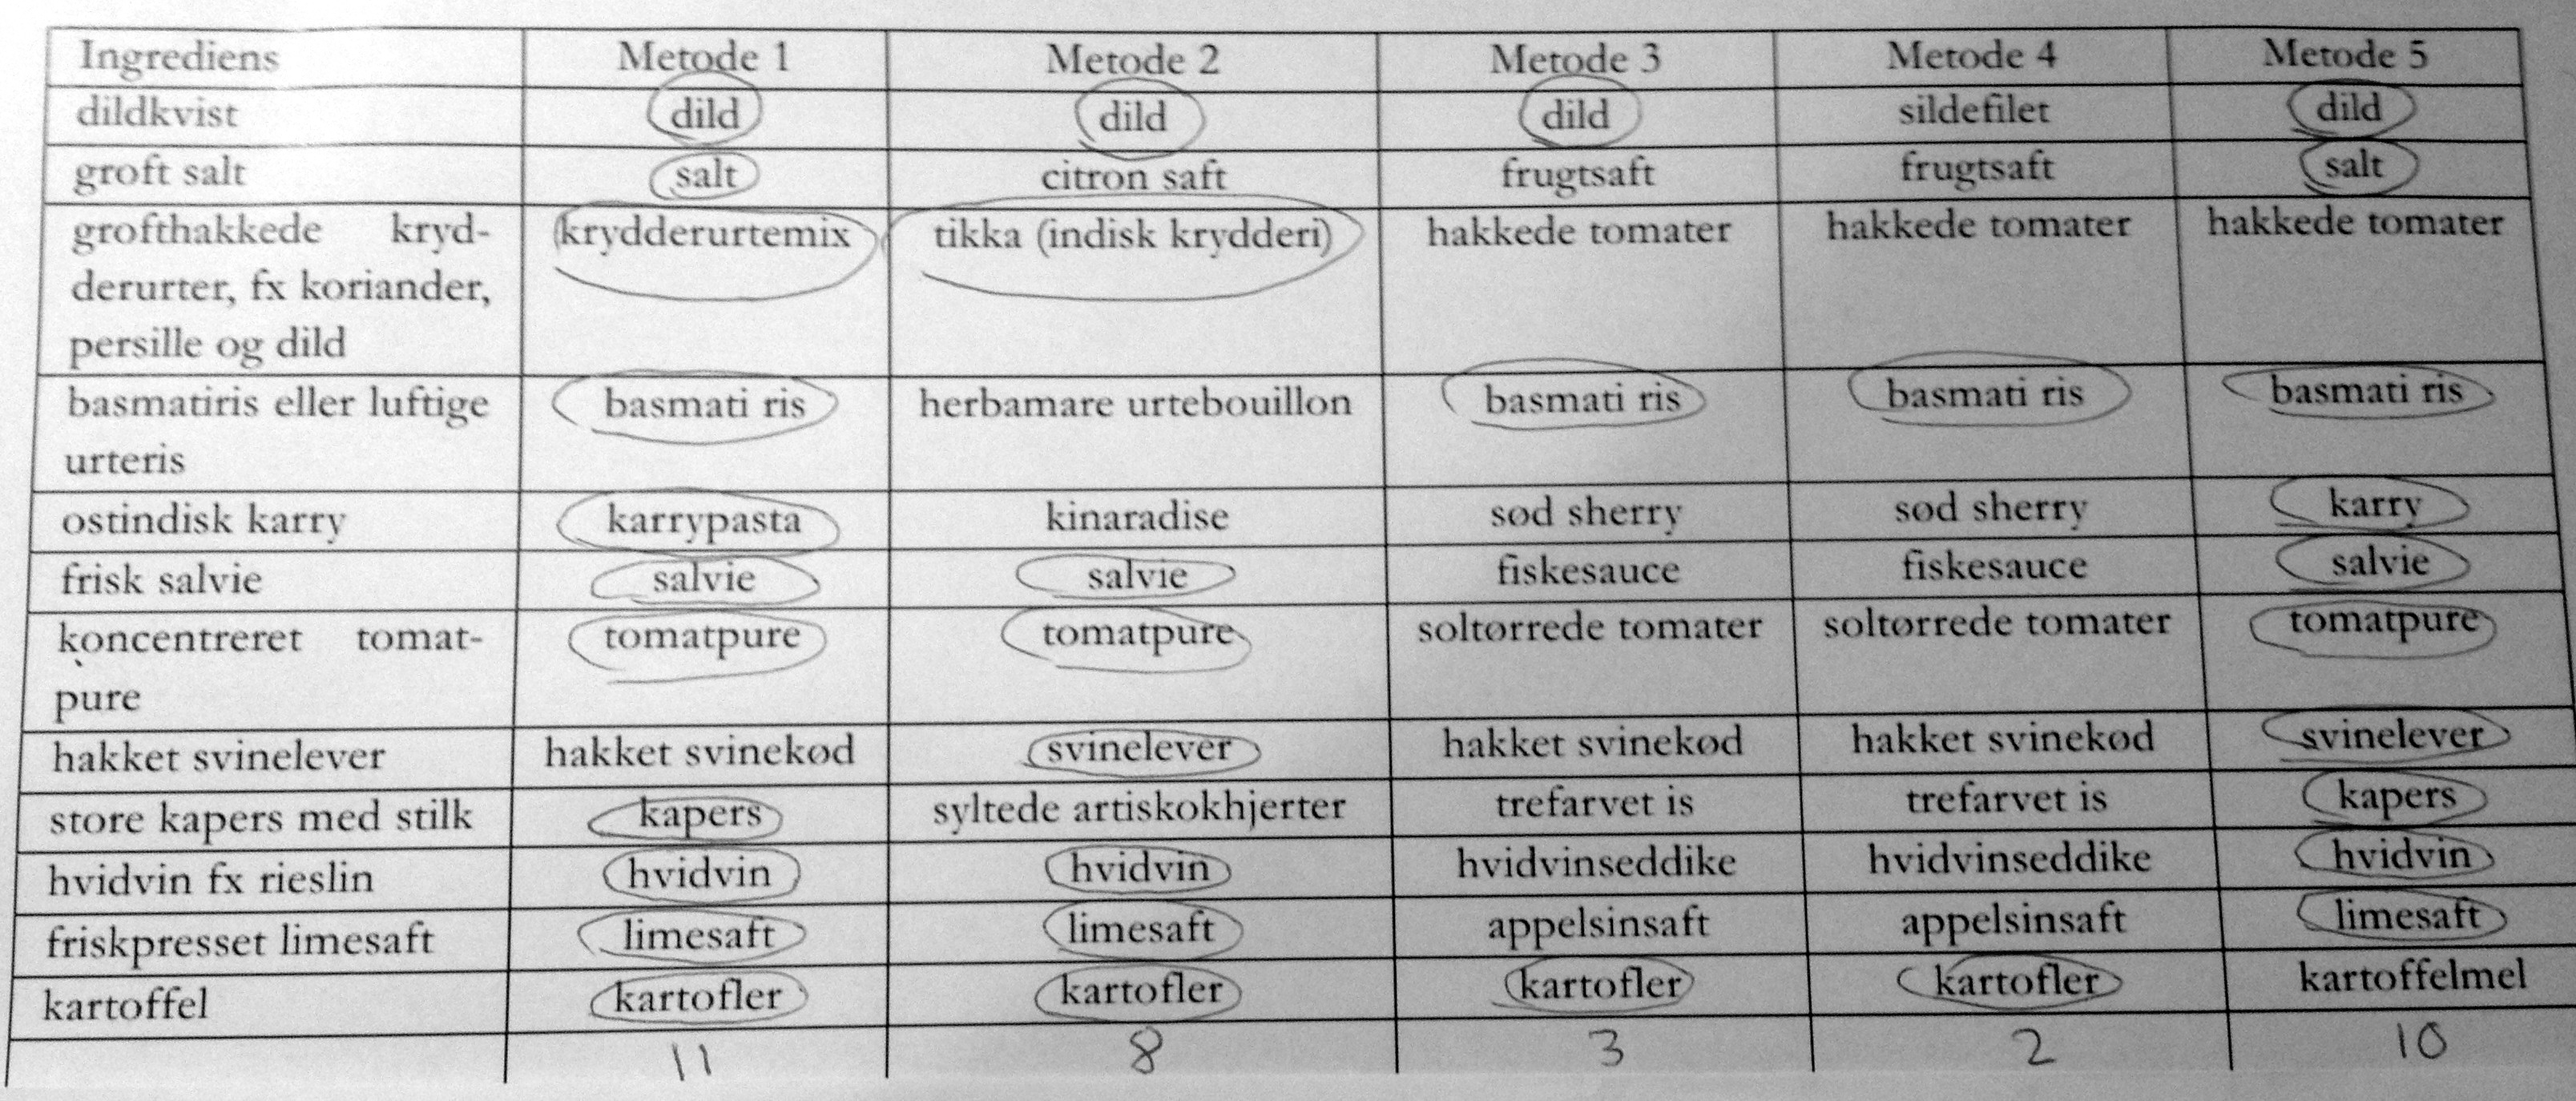
\includegraphics[width=0.8\textwidth]{billeder/valgafmappingmetode.jpg}
\capt{Informanterne satte ring om de mappings, de mente var korrekte. }
\end{figure}


\end{document}
